\section{Output Amplifier and Output}

\begin{figure}[H]
\centering
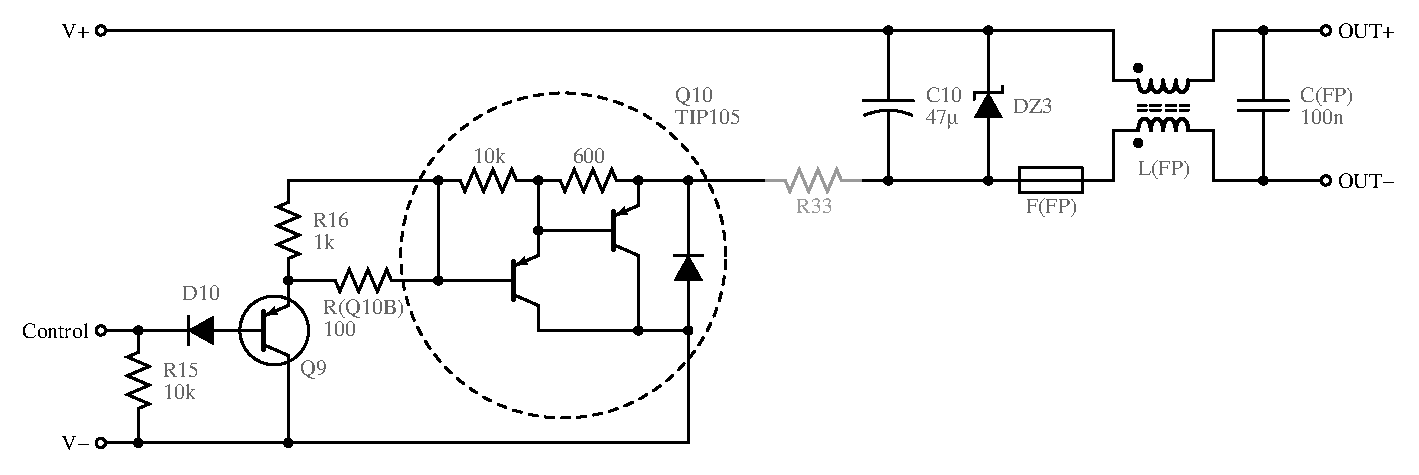
\includegraphics[width=5in]{sch/output}
\caption{Output sub-schematic}
\label{fig:output}
\end{figure}

\begin{multicols}{2}

The output amplifier buffers the signal from the voltage error amplifier, so
that it can supply the 500~mA output current. This is a simple circuit,
consisting of three emitter followers chained in a Darlington configuration.

The control signal is a current, not a voltage, so it is passed into
\texttt{R15} to convert it to voltage by Ohm's law. \texttt{D10} allows
current to sink out of \texttt{Q9}'s base, but prevents \texttt{Q9} from
being reverse-biased if a voltage is applied externally to the output.
\texttt{Q9} feeds \texttt{Q10}, which is a simple integrated circuit containing
two PNP transistors in a Darlington pair, the resistors connecting them, and a
diode from collector to emitter. This diode is also used for protection: if
a voltage is applied to the output while the PS-1 is unpowered, the diode will
allow this voltage to power the circuitry, developing proper bias voltages in
the system and protecting it from harm.

\texttt{C10} stores output charge, improving the transient response of the
power supply, and is also necessary for stability of the control loop.

\subsubsection{Parasitic Oscillators}
\texttt{R(Q10B)} is a ``base stopper'' resistor%
\footnote{If one wanted to research this topic further, one would find the
search term ``grid stopper'' more fruitful.}.
This resistor is installed directly at the base pin of \texttt{Q10}
(which is mounted off the board on wires). It forms an R-C low pass filter
with the tranistor's inherent base capacitance. This performs two functions.
First, it filters away any radio interference picked up by the wires, so that
this interference is not amplified and conducted to the output. Second, it
isolates the inductance of the wire from the transistor's base, preventing
an unintentional, parasitic Colpitts or Clapp oscillator from being formed from
the transistor and surrounding parasitics.

\subsubsection{Output Filter}
\texttt{L(FP)} and \texttt{C(FP)}, wired off-board, form a simple output
filter. This is not actually meant to filter the current on its way out, to
improve conditions for the DUT, but actually the reverse: if the DUT generates
any high-frequency currents, or if the test leads act as antennas and pick up
any high-frequency signals, they will block them from being absorbed by and
affecting the internal circuits. Capacitor \texttt{C(FP)} will shunt off any
differential currents from one wire to the other, and common-mode choke
\texttt{L(FP)} will block any common-mode (equal polarity in both wires)
currents.

\subsubsection{Output Protection}
In addition to the myriad small circuit additions (mostly diodes) already
described which protect the output in case of overload, there are two specific,
dedicated output protection devices.

\texttt{DZ3} is a transient voltage suppression (TVS) diode. In the PS-1H
model, it is a Vishay SMCJ30A. This is a form of Zener (actually avalanche)
diode, designed not to conduct at all up to 30~V, to begin conducting no higher
than 48.4~V, and to be able to withstand pulse currents of up to 31~A. Just
like a normal Zener diode, it will always conduct in the forward direction
(a negative voltage applied to the output) If an excessive voltage overload
applied, \texttt{DZ3} will crowbar it, blowing fuse \texttt{F(FP)} and
protecting the PS-1. The circuit is capable of directly withstanding overloads
up to this point without requiring the fuse to be blown.

\end{multicols}
